\documentclass[11pt, a4paper]{scrartcl}

\usepackage[left=3cm, right=3cm, top=3cm, bottom=3cm]{geometry}
\usepackage{graphicx}
\usepackage{array}
\usepackage{amsmath}


\newcommand{\git}{\mathbin{
  \mathchoice{/\mkern-6mu/}% \displaystyle
    {/\mkern-6mu/}% \textstyle
    {/\mkern-5mu/}% \scriptstyle
    {/\mkern-5mu/}}}% \scriptscriptstyle


\title{Monte Carlo Methods - Sheet 5}
\subtitle{XY Model: Hyprid-Monte-Carlo Algorithm}
\author{Tobias Sizmann}

\begin{document}
\maketitle
\textit{The blind frog lept out of its home to find food. It could sniff the food and most of the time found something acceptable (to eat). Also, it always found its way back home exactly (up to machine precision), since the frog is a symplectic frog - how convenient}
\section{Introduction}
    The XY-Model has - unlike the Ising Model - a continuous phase space. On first sight this might complicate things. However, it turns out that continuity gives rise to differentiation and therefore continuous dynamics - ultimatively leading to the hybrid method of molecular dynamics and Monte-Carlo. The goal hasn't changed with the XY-Model, namely sample the phase space of the physical problem following the importance given by the Boltzmann distribution as efficiently as possible. Concretely, the value to optimize is the number of statistically independent configurations per computer time. This problem becomes particularly difficult at critical parameters, here the critical temperature. Local algorithms like the Metropolis algorithm suffer from slowing down, which in turn motivate the design of global algorithms like the Wolff algorithm or in the case of this work the Hybrid-Monte-Carlo algorithm (HMC). The HMC uses equations of motion (EoM) derived from a specially designed guidance Hamiltonian to create proposal configurations that should in principal be guaranteed to be accepted. I.e. one has a new configuration with a finite difference to the seed configuration with every iteration of the algorithm. Numerical errors on the integration of the EoM however reduce the acceptance probability. The numerical errors are controlled by the integrator in use. In our case the integrator will be the leapfrog method. This numerical scheme is symplectic which is required to ensure detailed balance of the algorithm. Choosing the initial guidance momenta randomly ensures ergodicity as well.

\section{Finding optimal integration parameters}
    As already mentioned, acceptance rate and consequently (and directly) autocorrelation time are dependent on the properties of the integration process. In our case the integration scheme is parameterized by two parameters: The stepsize $dt$ and the number of leaps $n$. The choice of these parameters determines the efficiency of the HMC. This can be quickly understood when considering the limits. For $dt \rightarrow 0$ the acceptance rate becomes 1 as the guidance Hamiltonian doesn't change. However, the proposal configuration will become identical to its seed configuration and therefore the autocorrelation diverges and the data is useless. For $dt \rightarrow \infty$ the guidance Hamiltonian will change arbitrarily much due to integration errors and acceptance rate will converge to zero. No configurations will be accepted and once again the autocorrelation diverges. For $n \rightarrow \infty$ the integration errors once again diverge and therefore the autocorrelation does to. We can conclude that the optimum lies somewhere in the finite region. To find the optimal set of parameters the dependence of the efficiency on the parameters will be plotted and discussed. Three cases have been considered: Optimal $dt$ and $n$ for low temperature $T=0.67$ and for high temperature $T=3.33$ and optimal $dt$ for $n = 1$ over various temperatures.
\subsection{Low temperature $T = 0.67$}
    \begin{figure}
    \begin{centering}
        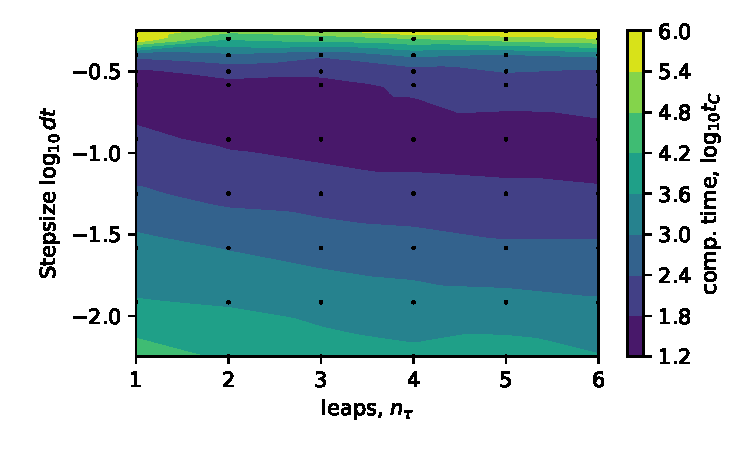
\includegraphics{low_T.pdf}
        \caption{\textbf{Dependence of efficiency on stepsize and number of steps at $T = 0.67$: } Plotted is a linearly interpolated contour heatmap of computer time per statistically independent configuration over stepsize $dt$ and number of steps $n$. Each black point resembles a sample with 100000 thermalized configurations on a 16 by 16 grid.}
    \end{centering}
    \label{lowT}
    \end{figure}
    Samples with 100000 configurations each have been generated on a 16 by 16 lattice and thermalized. The autocorrelation of the energy data $\tau_{int, E}$ has been calculated and an estimate for the computer time per independent configuration $t_c$ has been made using the formula $2*\tau_{int, E} * n$. A threshold for the maximum computer time estimate has been set to 100000 since any value beyond that can only be interpreted as a lower bound due to the length of each sample. The results are depicted in fig. \ref{lowT} employing a linearly interpolated contour heatmap to guide the eye. Actual measurement points are denoted by the small black dots in the plot. The divergence for high and low $dt$ are clearly visible. The optimal parameters seem to follow a pattern. For higher number of integration steps $n$ the stepsize $dt$ should be choosen lower. The reason to this is that with higher stepsize the integration error adds up more. Using a lower stepsize leads to a more precise trajectory. The efficiency stays roughly the same since the higher computation time is compensated by the lower correlation between two configurations.

    Note that in principal a true minimum rather than just a valley could exist for a higher number of steps than 7. Also note that - while for fixed $dt$ the computer time will diverge for $n \rightarrow \infty$ in a trivial way - it will also diverge for the path following valley. The reason for that is that the autocorrelation time cannot get better than 1 but the number of steps diverges and so does the computer time. One might even wonder if the autocorrelation oscillates if the system has some sort of oscillation, i.e., the guidance EoM return a periodic trajectory in phase space with the same frequency for any set of initial conditions.

    From the plot the optimal $dt$ for $n = 1$ is $10^{-0.6 \pm 0.2}$ where the error has been estimated roughly from the logarithmic measurement spacing.

\subsection{High temperature $T = 3.33$}
    \begin{figure}
    \begin{centering}
        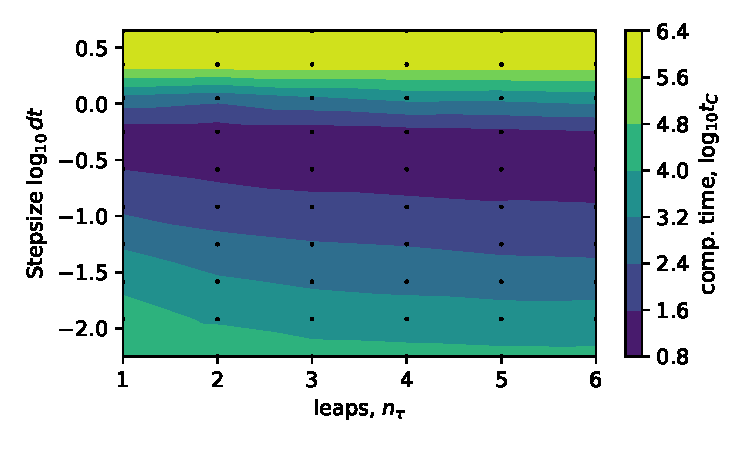
\includegraphics{high_T.pdf}
        \caption{\textbf{Dependence of efficiency on stepsize and number of steps at $T = 3.33$: } This plot is completely analogous to fig. \ref{lowT} except for the temperature.}
    \end{centering}
    \label{highT}
    \end{figure}
    The results for this temperature are depicted in fig. \ref{highT}. The plot has been created completely analogous to sec. 2.1 with the only exception being the higher temperature. Qualitatively the data looks the same and therefore no new discussion of the limits is made. There is an important difference however. The optimal $dt$ for a $n = 1$ is $10^{-0.35 \pm 0.2}$ and therefore significantly larger. For higher temperatures the difference in the guidance Hamiltonian and therefore the integration error has a less severe impact on the acceptance ratio. In the limit $T \rightarrow \infty$ the acceptance rate becomes $1$. This can be exploited by increasing $dt$ a bit and subsequently decreasing the autocorrelation. This motivates the next section where the $T$-dependence of $dt$ for a fixed $n = 1$ is examined more closely.
\subsection{Temperature dependence of $dt$}
    \begin{figure}
    \begin{centering}
        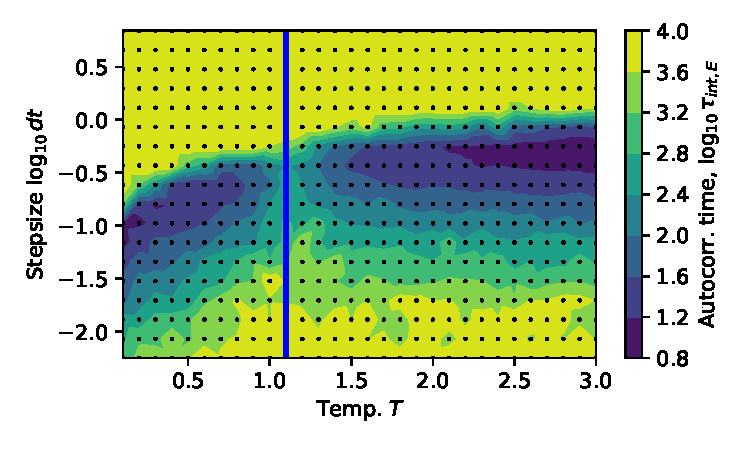
\includegraphics{dt_over_T.pdf}
        \caption{\textbf{Dependence of stepsize on temperature for fixed number of steps: } Plotted is the autocorrelation time $\tau_{int, E}$ for thermalized samples generated on a 16 by 16 grid with fixed number of integration steps $n = 1$. The data has been linearly interpolated and plotted as a contour heatmap to guide the eye. The black points denote the measurements. Each measurement is done on 100000 configurations. The blue line denotes the critical temperature of the XY-Model.}
    \end{centering}
    \label{dt_over_T}
    \end{figure}
    In this section the dependence of $dt$ on the temperature $T$ for fixed $n = 1$ is examined quantitatively. The results are depicted in fig. \ref{dt_over_T}. For $T \rightarrow 0$ the optimal $dt$ converges to $0$ as well. This follows the same reasoning as from sec. 2.2: In order to keep the acceptance rate high, the integration error must converge towards $0$ for $T \rightarrow 0$. An interesting idea for future work is the "true" analytical dependence.

    Note, that the autocorrelation increases in the critical region. This suggests the even the HMC as a global algorithm still is effected in some way by critical slowing down. An analysis on how this effect arises could be an interesting topic for future work. (Or am I missing something completely obvious here?)

\section{Temperature dependence of the magnetisation}
    \begin{figure}
    \begin{centering}
        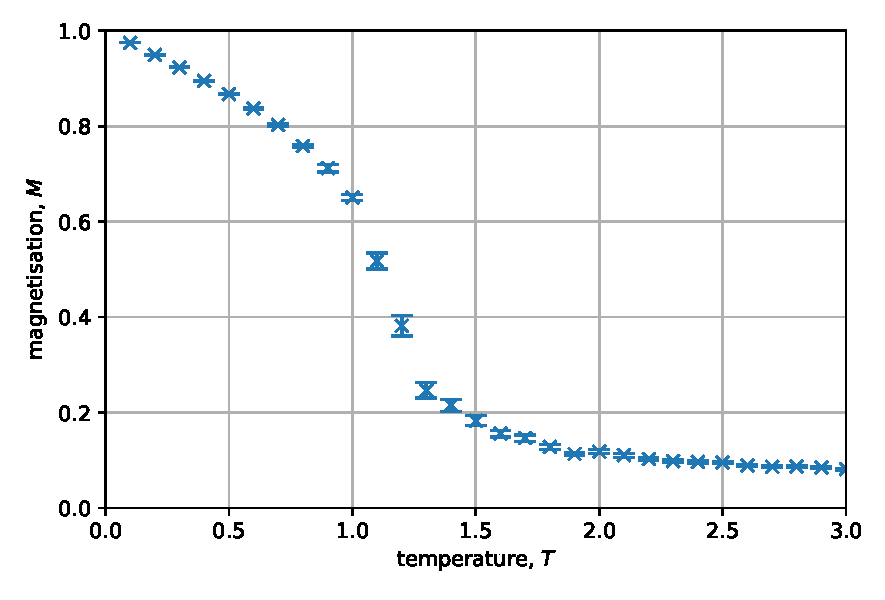
\includegraphics{m_over_T.pdf}
        \caption{\textbf{Dependence of magnetisation on temperature: } Plotted is the magnetisation over temperature. Each data point has been evaluated by a HMC sample with 100000 configurations on a 16 by 16 grid. The integration variables have been set to $dt = 0.1$ and $n = 1$.}
    \end{centering}
    \label{m_over_T}
    \end{figure}
    As in the Ising model the temperature dependence of the magnetisation is of scientific interest. To this end a set of samples with 100000 configurations each on a 16 by 16 lattice has been generated. The same integration parameters have been used for all temperatures, namely $dt = 0.1$ and $n = 1$. While they are inefficient for certain ranges of temperatures (see Sec 2.3) they have proven to produce acceptable results in realistic computation time across the range of interesting temperatures. The results are depicted in fig. \ref{m_over_T}. The curve resembles qualitatively the one from the Ising model. The critical temperature is different however. It has been estimated to be at $T = 1.1 \pm 0.1$ using data on standard deviation of the magnetisation. 
\end{document}
